\chapter{Dai riconoscitori agli interpreti}

\subsubsection{Dai puri riconoscitori...}
Finora si sono considerati soltanto \textit{puri riconoscitori}, che:
\begin{itemize}
    \item accettano in ingresso una stringa di caratteri
    \item riconoscono se essa appartiene a un linguaggio
\end{itemize}

\begin{figure}[H]
    \centering
    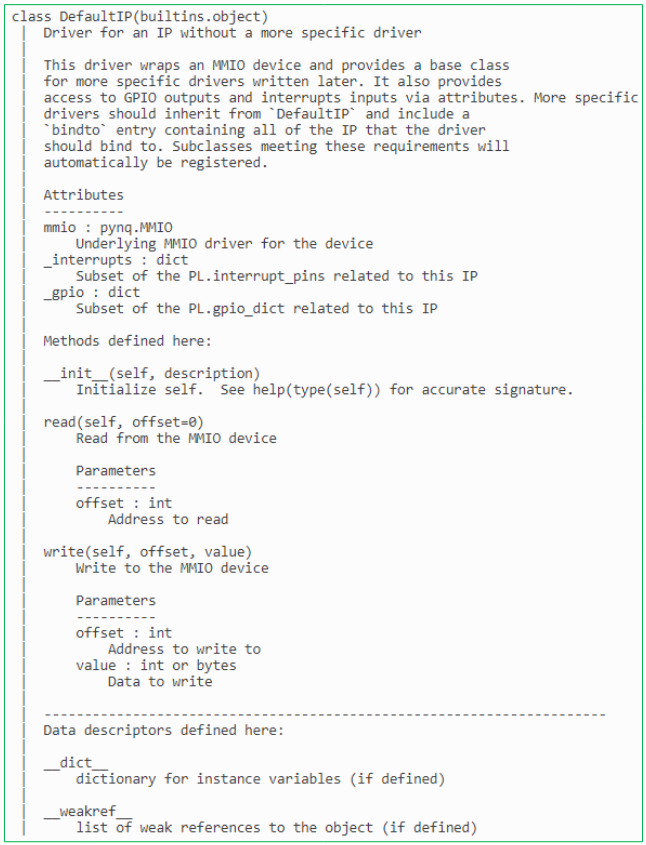
\includegraphics[width=0.8\textwidth]{/home/riccardoob/appunti/linguaggi/images/18.png}
\end{figure}

La risposta è sempre di tipo booleano, non ha importanza \textit{come} si arriva a stabilire la correttezza.

\subsubsection{...agli interpreti}
Un \textbf{interprete} è più di un puro riconoscitore, riconosce una stringa ma esegue anche azioni in base al significato (\textit{semantica}) della frase analizzata.

In questo caso diventa importante la \underline{sequenza di derivazione}.

\section{Interprete}

\subsection{Struttura}
Un interpreste è solitamente basasto su due componenti:
\begin{itemize}
    \item analizzatore lessicale, \textbf{scanner} o \textit{lexer}
    \item analizzatore sintattico-semantico, \textbf{parser}
\end{itemize}

\begin{figure}[H]
    \centering
    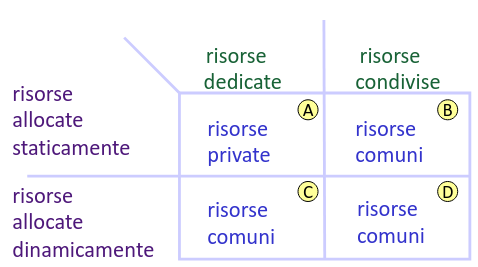
\includegraphics[width=0.8\textwidth]{/home/riccardoob/appunti/linguaggi/images/19.png}
\end{figure}

Lo scanner analizza le parti \textit{regolari} dei linguaggi, fornendo al parser singoli token già aggregati.

Il parser riceve dallo scanner i token, considerati come elementi terminali del suo linguaggio per valutare la correttezza della loro sequenza: opera sulle parti context free del linguaggio.

\subsection{Analisi lessicale}
L'analisi lessicale è la fase in cui si individuano le singole parole (token) che compongono la frase. Questa azione viene svolta raggruppando i singoli caratteri dell'input secondo \textbf{produzioni regolari} associate alle diverse possibili \textbf{categorie} lessicali.

L'analizzatore lessicale categorizza i token osservando in quale stato finale del RSF si ritrova.

\begin{figure}[H]
    \centering
    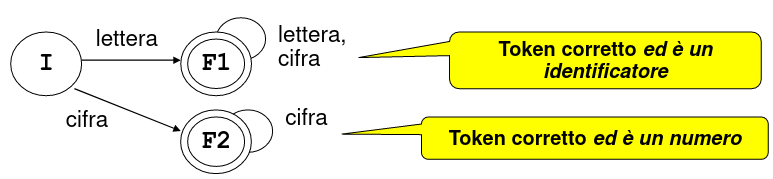
\includegraphics[width=0.8\textwidth]{/home/riccardoob/appunti/linguaggi/images/20.png}
\end{figure}

\subsection{Parole chiave}
Cablare ogni dettaglio nella struttura del RSF non è una buona strategia in quanto renderebbe estremamente complicato il riconoscitore.

\begin{figure}[H]
    \caption{Esempio riconoscimento identificatore if}
    \centering
    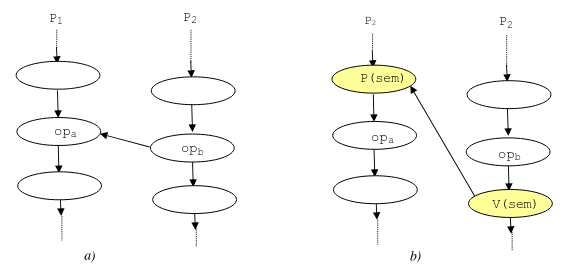
\includegraphics[width=0.7\textwidth]{/home/riccardoob/appunti/linguaggi/images/21.png}
\end{figure}

\subsection{Tabelle}
Per evitare di cablare le parole chiave, simboli etc. nella struttura del RSF, conviene agire diversamente:
\begin{itemize}
    \item categorizzare prima le parole chiave come identificatori
    \item ricategorizzare poi consultando opportune tabelle che incapsulano il dettaglio del linguaggio
    \begin{itemize}
        \item tabella \textit{parole chiave}
        \item tabella \textit{simboli}
    \end{itemize}
\end{itemize}

\subsection{Analisi sintattica top-down}
In caso di grammatiche $LL(1)$, una tecnica semplice per costruire il riconoscitore è l'analisi top-down ricorsiva discendente.

Per passare da un puro riconoscitore a un interprete occorre propagare qualcosa di più di un si o no, come ad esempio un \textbf{albero}, per una valutazione differita.

\section{Caso di studio - espressioni aritmetiche}
Si supponga di voler riconoscere espressioni aritmetiche con le quattro operazioni \textbf{+ * - /}.

\begin{figure}[H]
    \centering
    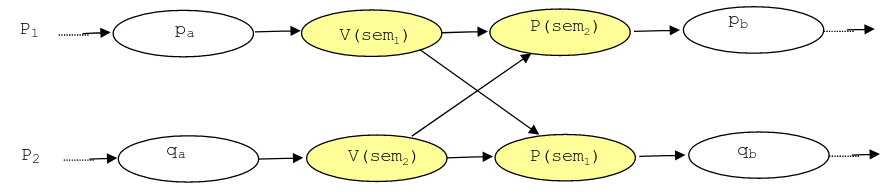
\includegraphics[width=0.8\textwidth]{/home/riccardoob/appunti/linguaggi/images/22.png}
\end{figure}

Un puro riconoscitore deve solo dire se sono corrette, ma un interprete deve anche dire:
\begin{itemize}
    \item se il dominio sono gli \textit{interi} il risultato può essere un valore int
    \item se il dominio sono i \textit{reali} il risultato può essere un valora double
    \item se l'obiettivo è la \textit{valutazione differita}, il risultato può essere un opportuno oggetto (albero)
\end{itemize}

\subsection{Analisi del dominio}

\subsubsection{Sintassi}
La notazione classica insegnata identifica i quattro operatori con i seguenti simboli: $+$, $-$, $\times$, $:$.

Sono stati sostituiti dagli informatici con $+$, $-$, $*$, $/$, spesso vengono anche usate le parentesi per esprimere una priorità associativa.

\subsubsection{Semantica}
Nel dominio aritmetico usuale:
\begin{itemize}
    \item i \textit{valori numerici} si assumono espressi in notazione \textbf{posizionale} su base dieci
    \item il significato inteso dei quattro \textit{operatori} è quello di somma, sottrazione, moltiplicazione, divisione
    \item si denotano le nozioni di priorità e associatività
    \begin{itemize}
        \item \textbf{priorità} fra operatori diversi, moltiplicativi prioritari su quelli additivi
        \item \textbf{associatività} tra operatori equiprioritari, solitamente si associa a sinistra
    \end{itemize}
\end{itemize}

\subsection{Grammatica per le espressioni}
Consideriamo il linguaggio $E(G)$ relativo alla seguente grammatica per espressioni aritmetiche;
\setlist{nosep}
\begin{itemize}[label={}]
    \item $\texttt{VN} = \{ \texttt{EXP}\}$
    \item $\texttt{VT} = \{+, *, -, :, \texttt{num}\}$
    \item $S = \texttt{EXP}$
    \item $P = \{$
    \begin{itemize}[label={}]
        \item $\texttt{EXP} := \texttt{EXP} + \texttt{EXP}$
        \item $\texttt{EXP} := \texttt{EXP} - \texttt{EXP}$
        \item $\texttt{EXP} := \texttt{EXP} * \texttt{EXP}$
        \item $\texttt{EXP} := \texttt{EXP} : \texttt{EXP}$
        \item $\texttt{EXP} := \texttt{num}$ 
    \end{itemize}
    \item $\}$
\end{itemize}
\setlist{}
É una grammatica ambigua, la semantica è informale: se \texttt{EXP} è un numero, l'espressione denota un intero e il valore dell'espression coincide con quello del numero.

\subsection{Una grammatica a "strati"}
É possibile dare una struttura \textit{gerarchica} alle espressioni, esprimendo così intrinsicamente priorità e associatività degli operatori.
\setlist{nosep}
\begin{itemize}[label={}]
    \item $\texttt{VN} = \{ \texttt{EXP}, \texttt{TERM}, \texttt{FACTOR}\}$
    \item $\texttt{VT} = \{+, *, -, :, (, ), \texttt{num}\}$
    \item $S = \texttt{EXP}$
    \item $P = \{$
    \begin{itemize}[label={}]
        \item $\texttt{EXP} := \texttt{TERM}$
        \item $\texttt{EXP} := \texttt{EXP} + \texttt{TERM}$
        \item $\texttt{EXP} := \texttt{EXP} - \texttt{TERM}$
        \item $\texttt{TERM} := \texttt{FACTOR}$
        \item $\texttt{TERM} := \texttt{TERM} * \texttt{FACTOR}$
        \item $\texttt{TERM} := \texttt{TERM} : \texttt{FACTOR}$
        \item $\texttt{FACTOR} := \texttt{num}$
        \item $\texttt{FACTOR} := ( \texttt{EXP})$
    \end{itemize}
    \item $\}$
\end{itemize}
\setlist{}
Ogni strato considera \textit{terminali} gli elementi linguistici definiti in altri strati:
\begin{itemize}
    \item \texttt{EXP} considera terminali $+$, $-$ e \texttt{TERM}
    \item \texttt{TERM} considera terminali $*$, $:$ e \texttt{FACTOR}
    \item \texttt{FACTOR} considera terminali \texttt{num}, $($, $)$, e \texttt{EXP}
\end{itemize}

Le \textit{somme} e \textit{sottrazioni} aggregano i \underline{termini}, le \textit{moltiplicazioni} e \textit{divisioni} aggregano i \underline{fattori} e i \textit{fattori} sono entità \underline{atomiche}.

\begin{figure}[H]
    \caption{Priorità operatori}
    \centering
    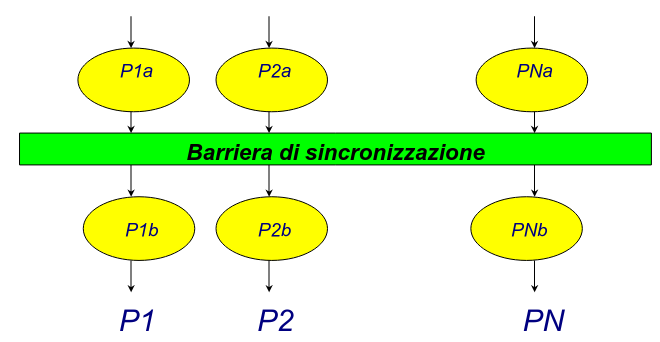
\includegraphics[width=0.8\textwidth]{/home/riccardoob/appunti/linguaggi/images/23.png}
\end{figure}

\subsubsection{Esempi}

\begin{multicols}{2}
    Frase:\\
    \noindent
    $(0111 + 0011) * 0010$\\
    Albero di derivazione
    \begin{multicolfigure}
        \centering
        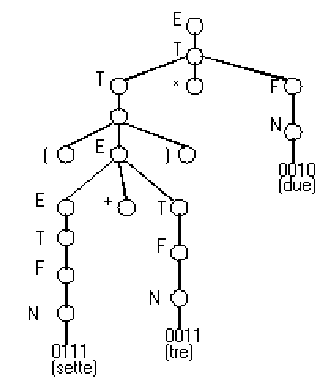
\includegraphics[width=0.7\textwidth]{/home/riccardoob/appunti/linguaggi/images/24.png}
    \end{multicolfigure}
    \columnbreak
    Frase:\\
    \noindent
    $0111 + 0011 + 0010$\\
    Albero di derivazione
    \begin{multicolfigure}
        \centering
        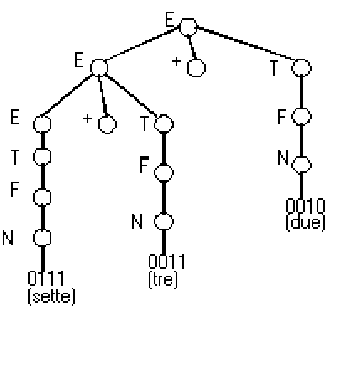
\includegraphics[width=0.7\textwidth]{/home/riccardoob/appunti/linguaggi/images/25.png}
    \end{multicolfigure}
\end{multicols}

La grammatica individuata è \textit{ricorsiva a sinistra} per esprimere la corretta associatività, tuttavia è incompatibile con l'analisi ricorsiva discendente, utile per la costruzione del parser.

\subsection{Variante 1 - Associativa a destra}
Se si riscrivono le regole in forma ricorsiva a destra, ovvero invertendo \texttt{TERM} e \texttt{EXP} e \texttt{FACTOR} e \texttt{TERM}, si otterrebbe una associatività inversa rispetto a quella usuale.

Ad esempio l'espressione $7 - 3 - 2$ verrebbe derivata come $7 - ( 3 - 2 )$ anziché come $( 7 - 3 ) - 2$.

\setlist{nosep}
\begin{itemize}[label={}]
    \item $\texttt{VN} = \{ \texttt{EXP}, \texttt{TERM}, \texttt{FACTOR}\}$
    \item $\texttt{VT} = \{+, *, -, :, (, ), \texttt{num}\}$
    \item $P = \{$
    \begin{itemize}[label={}]
        \item $\texttt{EXP} := \texttt{TERM}$
        \item $\texttt{EXP} := \texttt{TERM} + \texttt{EXP}$
        \item $\texttt{EXP} := \texttt{TERM} - \texttt{EXP}$
        \item $\texttt{TERM} := \texttt{FACTOR}$
        \item $\texttt{TERM} := \texttt{FACTOR} * \texttt{TERM}$
        \item $\texttt{TERM} := \texttt{FACTOR} : \texttt{TERM}$
        \item $\texttt{FACTOR} := \texttt{num}$
        \item $\texttt{FACTOR} := ( \texttt{EXP})$
    \end{itemize}
    \item $\}$
\end{itemize}
\setlist{}


\subsection{Variante 2 - Non associativa}
Si potrebbe anche fare a meno dell'associatività, mantenendo però lo stesso ordine di priorità. Queste regole non usano ricorsione, ne destra ne sinistra, risolvendo il problema \textit{obbligando a usare le parentesi}.

\setlist{nosep}
\begin{itemize}[label={}]
    \item $\texttt{VN} = \{ \texttt{EXP}, \texttt{TERM}, \texttt{FACTOR}\}$
    \item $\texttt{VT} = \{+, *, -, :, (, ), \texttt{num}\}$
    \item $P = \{$
    \begin{itemize}[label={}]
        \item $\texttt{EXP} := \texttt{TERM}$
        \item $\texttt{EXP} := \texttt{TERM} + \texttt{TERM}$
        \item $\texttt{EXP} := \texttt{TERM} - \texttt{TERM}$
        \item $\texttt{TERM} := \texttt{FACTOR}$
        \item $\texttt{TERM} := \texttt{FACTOR} * \texttt{FACTOR}$
        \item $\texttt{TERM} := \texttt{FACTOR} : \texttt{FACTOR}$
        \item $\texttt{FACTOR} := \texttt{num}$
        \item $\texttt{FACTOR} := ( \texttt{EXP})$
    \end{itemize}
    \item $\}$
\end{itemize}
\setlist{}

\section{Dalla grammtica al parser}
\subsection{Ricorsione sinista e analisi top-down}
Il riconoscitore è un PDA, perché la grammatica ha self-embedding, il problema è che la sintassi delle espressioni include produzioni \textit{ricorsive sinistra}, quindi questa non è una grammatica $LL(1)$.

\subsubsection{Trasformazione della grammatica}
Si procede riconsiderando i sotto-linguaggi generati dai diversi strati:
\setlist{nosep}
\begin{itemize}[label={}]
    \item $\texttt{L(EXP)} = \texttt{TERM} \pm \texttt{TERM} \pm \texttt{TERM} \dots$
    \item $\texttt{L(TERM)} = $*/:$ \texttt{FACTOR} $*/:$ \texttt{FACTOR} \dots$
    \item $\texttt{L(FACTOR)} = \texttt{num}\ |\ \texttt{(EXP)}$
\end{itemize}
\setlist{}

Continuiamo mappando le espressioni individuate seconda la notazione EBNF:
\setlist{nosep}
\begin{itemize}[label={}]
    \item \texttt{EXP} = \texttt{TERM} $\{(+ | -) \texttt{TERM}\}$
    \item \texttt{TERM} = \texttt{FACTOR} $\{(* | :) \texttt{FACTOR}\}$
\end{itemize}
\setlist{}
Queste regole non presentano più ricorsione esplicita, descrivono un processo computazionale iterativo.

Questa è una grammatica $LL(1)$, in quanto è analizzabile con una tecnica ricorsiva discendente e hanno start symbols set distinti.

Si può esplicitare inserendo un termine:
\setlist{nosep}
\begin{itemize}[label={}]
    \item \texttt{EXP} = \texttt{TERM} \texttt{AFTERTERM}
    \item \texttt{AFTERTERM} = $\varepsilon\ |\ +$\texttt{EXP}$\ |\ -$\texttt{EXP} 
    \item \texttt{TERM} = \texttt{FACTOR} \texttt{AFTERFACTOR}
    \item \texttt{AFTERFACTOR} = $\varepsilon\ |\ *$\texttt{TERM}$|\ :$\texttt{TERM}
\end{itemize}
\setlist{}
Questa è una grammatica $LL(1)$ ma è anche ricorsiva a destra, non verrà quindi utilizzata operativamente ma solo per la verifica $LL(1)$

\subsubsection{Schema parser}
Si effettua una analisi ricorsiva discendente:
\begin{itemize}
    \item procedura o funzione per ogni simbolo non terminale
    \item invocazione ricorsiva solo per il caso con self-embedding
\end{itemize}

Tutte le funzioni restituiscono un \textit{boolean}, nel caso di puro riconoscitore, oppure un valore o oggetto nel caso di parser completi con valutazione.

Ogni funzione dovrebbe terminare quando incontra un simbolo che non appartiene al sotto-linguaggio di sua pertinenza.

\begin{lstlisting}[language=java]
    public boolean parseExp() {
        boolean t1 = parseTerm();
        while (currentToken != null) {
            if (currentToken.equals("+"))
\end{lstlisting}

\textbf{\_\_\_\_\_\_\_\_\_\_\_\_\_\_\_\_\_\_\_\_\_\_\_\_\_\_\_\_\_\_\_\_\_\_\_\_\_\_\_\_\_\_\_\_\_\_\_\_\_\_\_inserisci codice slide 37-39\_\_\_\_\_\_\_\_\_\_\_\_\_\_\_\_\_\_\_\_\_\_\_\_\_\_\_\_\_\_\_\_\_\_\_\_\_\_\_\_\_\_\_\_\_\_\_\_\_\_\_}

\subsubsection{Una architettura di sistema}
Si passa ora a definira una architettura di supporto per il parser, come ad esempio concretizzare il concetto di \textbf{token} e astrarre lo scanner per leggere la stringa e definire il modello di interazione tra parser e scanner.

Si potrebbe, ad esempio, utilizzare una variabile privata \texttt{currentToken}, una classe \texttt{MyScanner} per tokenizzare la stringa e una classe \texttt{Token} che incapsula una stringa.

\textbf{\_\_\_\_\_\_\_\_\_\_\_\_\_\_\_\_\_\_\_\_\_\_\_\_\_\_\_\_\_\_\_\_\_\_\_\_\_\_\_\_\_\_\_\_\_\_\_\_\_\_\_inserire codice 42-46\_\_\_\_\_\_\_\_\_\_\_\_\_\_\_\_\_\_\_\_\_\_\_\_\_\_\_\_\_\_\_\_\_\_\_\_\_\_\_\_\_\_\_\_\_\_\_\_\_\_\_}

\section{Dal parser al valutatore}
Finora abbiamo definito come:
\begin{itemize}
    \item dato il \textit{linguaggio} desiderato, trovare una \textit{grammatica} adatta a descriverlo
    \item data la grammatica, scrivere un puro \textit{riconoscitore} per tale linguaggio
\end{itemize}
manca:
\begin{itemize}
    \item data la grammatica, scrivere un \textbf{parser} completo che effettui una \textbf{valutazione}
\end{itemize}
serve:
\begin{itemize}
    \item la specifica della semantica che il parser dovrà applicare
\end{itemize}

\subsection{Specificare la semantica}
É necessario un modo sistematico e formale stabilire con precisione il \textbf{significato} di ogni possibile frase di un linguaggio: se il linguaggio è \textit{infinito} serve una notazione finita applicabile a infinite frasi.

Un metodo può essere qello di definire una \textit{funzione di interpretazione}:
\begin{itemize}
    \item \underline{dominio}, ovvero il linguaggio
    \item \underline{codominio}, ovvero l'insieme dei possibili significati
\end{itemize}

\subsection{Semantica denatoziale}
Quando la semantica di un lingauggio è espressa in questo modo si parla di \textbf{semantica denotazionale}.

L'idea principale è quella di associare a ogni \textit{regola sintattica} una \textbf{regola semantica}.

Nel caso delle espressioni aritmetiche la sintassi prevede \texttt{Exp}, \texttt{Term} e \texttt{Factor}, quindi la semantica prevederà le funzioni \texttt{fExp}, \texttt{fTerm} e \texttt{fFactor}.

\begin{itemize}
    \item \texttt{fExpr(s)}
    \begin{itemize}
        \item \texttt{fTerm(s)} se \texttt{s} non contiene ne $+$ ne $-$
        \item \texttt{fExpr(s1)}$+$\texttt{fTerm(s2)}, se \texttt{s} ha la forma \texttt{s1}$+$\texttt{s2}
        \item \texttt{fExpr(s1)}$-$\texttt{fTerm(s2)}, se \texttt{s} ha la forma \texttt{s1}$-$\texttt{s2}
    \end{itemize}
    \item \texttt{fTerm(s)}
    \begin{itemize}
        \item \texttt{fFactor(s)} se \texttt{s} non contiene ne $*$ ne $:$
        \item \texttt{fTerm(s1)}$\times$\texttt{fFactor(s2)} se \texttt{s} ha la forma \texttt{s1}$*$\texttt{s2}
        \item \texttt{fTerm(s1)}$/$\texttt{fFactor(s2)} se \texttt{s} ha la forma \texttt{s1}$:$\texttt{s2}
    \end{itemize}
    \item \texttt{fFactor(s)}
    \begin{itemize}
        \item \texttt{fFactor(innerExp)} se \texttt{s} ha la forma \texttt{(innerExp)}
        \item \texttt{valueof(num)}, se \texttt{s} ha la forma \texttt{num}
    \end{itemize}
\end{itemize}

\begin{figure}[H]
    \centering
    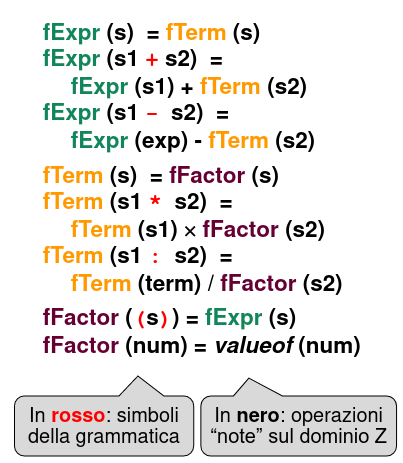
\includegraphics[width=0.4\textwidth]{/home/riccardoob/appunti/linguaggi/images/32.png}
\end{figure}
\subsubsection{Esempio}
\begin{figure}[H]
    \centering
    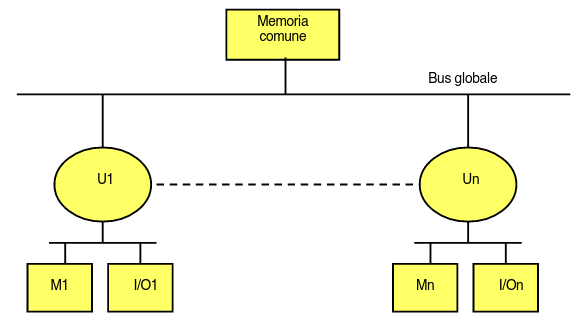
\includegraphics[width=0.7\textwidth]{/home/riccardoob/appunti/linguaggi/images/33.png}
\end{figure}

\subsubsection{Schema interprete}
Ogni funzione analizza il sotto-linguaggio di pertinenza:
\begin{itemize}
    \item \texttt{parseExp} analizza \texttt{L(EXP)}, per il quale $+$, $-$ e \texttt{TERM} sono l'alfabeto terminale
    \item \texttt{parseTerm} analizza \texttt{L(TERM)}, per il quale $*$, $:$ e \texttt{FACTOR} sono l'alfabeto terminale
    \item \texttt{parseFactor} analizza \texttt{L(FACTOR)}, il cui alfabeto terminale è costituito da $($, $)$ e \texttt{EXP}
\end{itemize}

\textbf{\_\_\_\_\_\_\_\_\_\_\_\_\_\_\_\_\_\_\_\_\_\_\_\_\_\_\_\_\_\_\_\_\_\_\_\_\_\_\_\_\_\_\_\_\_\_\_\_\_\_\_inserisci codice slide 64-67\_\_\_\_\_\_\_\_\_\_\_\_\_\_\_\_\_\_\_\_\_\_\_\_\_\_\_\_\_\_\_\_\_\_\_\_\_\_\_\_\_\_\_\_\_\_\_\_\_\_\_}
\subsection{Elevamento a potenza}
Se si volesse aggiungere l'elevamento a potenza?

Si introduce l'operatore \texttt{\^}, che denota un elevamento a potenza: $3*4^2$ si scrive \texttt{3*4\^{}2} 

Questo operatore ha priorità maggiore di tutti gli altri e si considera la sua associatività è a destra, ovvero si interpreta $4^{2^3}$ o \texttt{4\^{}2\^{}3} come $4^8$.

Si aggiunge un nuovo "strato" alla grammatica a strati definita in precedenza:
\begin{figure}[H]
    \centering
    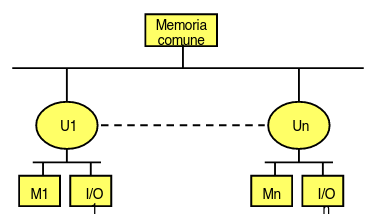
\includegraphics[width=0.4\textwidth]{/home/riccardoob/appunti/linguaggi/images/34.png}
\end{figure}

\textbf{\_\_\_\_\_\_\_\_\_\_\_\_\_\_\_\_\_\_\_\_\_\_\_\_\_\_\_\_\_\_\_\_\_\_\_\_\_\_\_\_\_\_\_\_\_\_\_\_\_\_\_inserisci codice slide 70-72\_\_\_\_\_\_\_\_\_\_\_\_\_\_\_\_\_\_\_\_\_\_\_\_\_\_\_\_\_\_\_\_\_\_\_\_\_\_\_\_\_\_\_\_\_\_\_\_\_\_\_}

\section{Rappresentare le frasi}
Manca soltanto una rappresentazione intermedia della frase interpretata per poter "risolverla" successivamente, qui entrano in gioco gi \textbf{alberi sintattici}.

\subsection{Alberi sintattici astratti}
Si potrebbe usare dirattamente l'\textit{albero di derivazione}, ma darebbe luogo a una rappresentazione ridondante.

Conviene adottare un albero più \textit{compatto}, che contenga solo i nodi indispensabili, la soluzione è il \textbf{Abstract Syntax Tree} (AST).

Tipologie di nodi non indispensabili:
\begin{itemize}
    \item i nodi terminali (foglie) non legati a niente di significativo sono ridondanti e possono essere ignorati, le foglie 
    \item le foglie che esauriscono la loro funzione dopo il parser, nelle espressioni le parentesi
    \item le foglie che hanno un unico nodo figlio
\end{itemize}

\begin{multicols}{2}    
    \begin{multicolfigure}
        \centering
        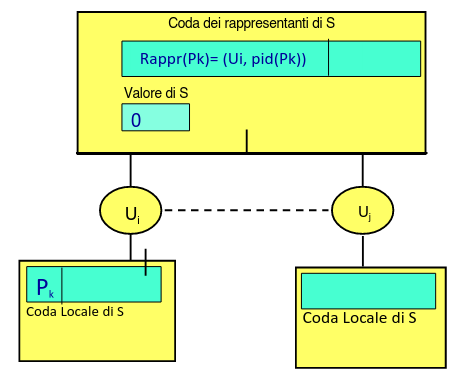
\includegraphics[width=0.5\textwidth]{/home/riccardoob/appunti/linguaggi/images/35.png}
    \end{multicolfigure}
    \columnbreak
    \begin{multicolfigure}
        \centering
        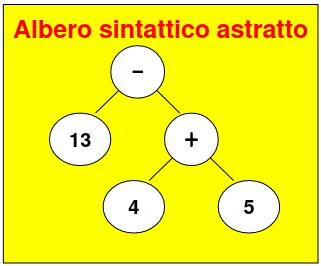
\includegraphics[width=0.5\textwidth]{/home/riccardoob/appunti/linguaggi/images/36.png}
    \end{multicolfigure}
\end{multicols}

\subsubsection{Esempio espressioni}

Nel caso delle espressioni, l'AST è così definito
\begin{itemize}
    \item ogni \textbf{operatore} è un nodo con due figli
    \begin{itemize}
        \item figlio sinistro è il primo operando
        \item figlio destro è il secondo operando
    \end{itemize}
    \item i valori numerici sono le foglie
\end{itemize}

La rappresentazione è sempre univoca, quindi la struttura dell'albero fornisce intrinsicamente l'ordine corretto di valutazione.

Si tenta ora di estendere il parser per generare l'opportuno AST, per farlo è necessario stabilire quali e quanti tipi di nodo diversi si hanno.

\begin{figure}[H]
    \centering
    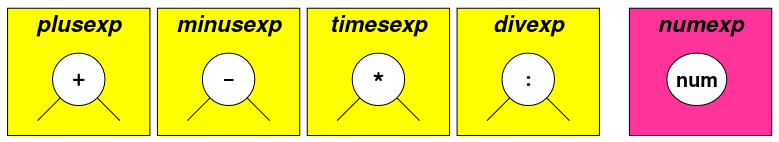
\includegraphics[width=0.6\textwidth]{/home/riccardoob/appunti/linguaggi/images/37.png}
\end{figure}

\subsection{Sintassi astratta}
Per descrivere formalmente questi nodi si utilizza una \textbf{sintassi astratta}, ad esempio i nodi in considerazione possono essere rappresentanti con la seguente sintassi astratta

\setlist{nosep}
\begin{itemize}[label={}]
    \item \texttt{EXP} = \texttt{EXP} $+$ \texttt{EXP}
    \item \texttt{EXP} = \texttt{EXP} $-$ \texttt{EXP}
    \item \texttt{EXP} = \texttt{EXP} $*$ \texttt{EXP}
    \item \texttt{EXP} = \texttt{EXP} $:$ \texttt{EXP}
    \item \texttt{EXP} = \texttt{num}
\end{itemize}
\setlist{}

\subsubsection{Una possibile implementazione dell'AST}
\textbf{\_\_\_\_\_\_\_\_\_\_\_\_\_\_\_\_\_\_\_\_\_\_\_\_\_\_\_\_\_\_\_\_\_\_\_\_\_\_\_\_\_\_\_\_\_\_\_\_\_\_\_inserisci codice slide 86-89\_\_\_\_\_\_\_\_\_\_\_\_\_\_\_\_\_\_\_\_\_\_\_\_\_\_\_\_\_\_\_\_\_\_\_\_\_\_\_\_\_\_\_\_\_\_\_\_\_\_\_}

Si passa ora alla nuova implementazione del parser che include la nuova architettura ad AST.

\textbf{\_\_\_\_\_\_\_\_\_\_\_\_\_\_\_\_\_\_\_\_\_\_\_\_\_\_\_\_\_\_\_\_\_\_\_\_\_\_\_\_\_\_\_\_\_\_\_\_\_\_\_inserisci codice slide 91-93\_\_\_\_\_\_\_\_\_\_\_\_\_\_\_\_\_\_\_\_\_\_\_\_\_\_\_\_\_\_\_\_\_\_\_\_\_\_\_\_\_\_\_\_\_\_\_\_\_\_\_}

\section{Architettura interprete}
\begin{figure}[H]
    \centering
    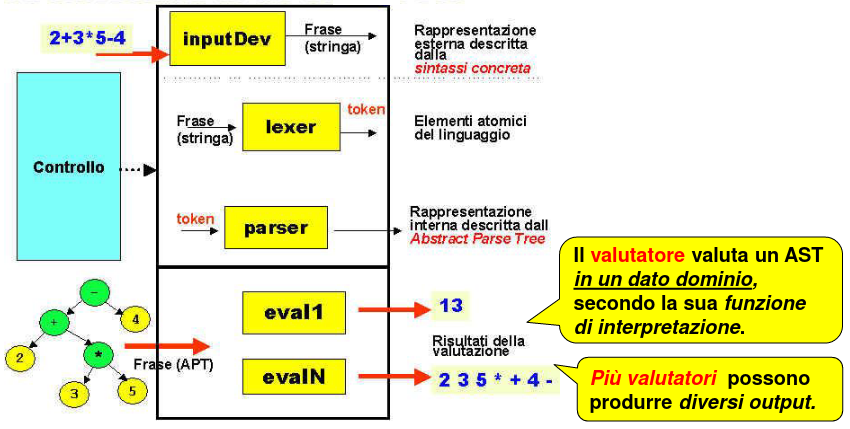
\includegraphics[width=0.8\textwidth]{/home/riccardoob/appunti/linguaggi/images/40.png}
\end{figure}
Si è arrivati al punto nel quale sono state definite strategie per:
\begin{itemize}
    \item dato il linguaggio desiderato, trovare una \textit{grammatica} adatta
    \item data la grammatica, scrivere il \textit{puro riconoscitore} per il linguaggio
    \item data la grammatica, scrivere un \textit{parser} completo che valuti e generi l'albero
\end{itemize}

manca da \textbf{valutare l'albero sintattico} dopo la sua generazione.

\section{Valutazione di alberi}
Esistono diverse modalità per analizzare una albero, la teoria degli alberi introduce il concetto di \underline{visita}:
\begin{itemize}
    \item \textit{pre-order}, radice $\rightarrow$ figli (da sx a dx)
    \item \textit{post-order}, figli (da sx a dx) $\rightarrow$, radice
    \item \textit{in-order}, figlio sx $\rightarrow$ radice $\rightarrow$ figlio dx
\end{itemize}

Nel nostro dominio delle espressioni aritmetiche, queste metodologie si traducono in:
\begin{itemize}
    \item notazione \textbf{prefissa}
    \item notazione \textbf{postfissa}
    \item notazione \textbf{infissa} classica
\end{itemize}

Con la notazione postfissa si presta perfettamente alla traduzione in codice per un elaboratore, in quanto fornisce prima gli operandi e successivamente cosa farne.

Idealmente si caricherebbero gli operandi su un registro, ma essendo questi limitati si utilizza lo \textbf{stack}.

Evoluzione dello stack:
\begin{multicols}{2}
    \begin{multicolfigure}
        \centering
        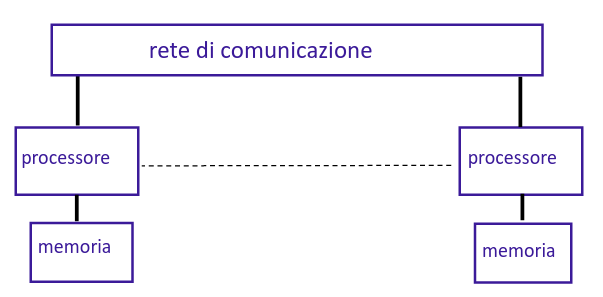
\includegraphics[width=0.45\textwidth]{/home/riccardoob/appunti/linguaggi/images/38.png}
    \end{multicolfigure}
    
    \begin{multicolfigure}
        \centering
        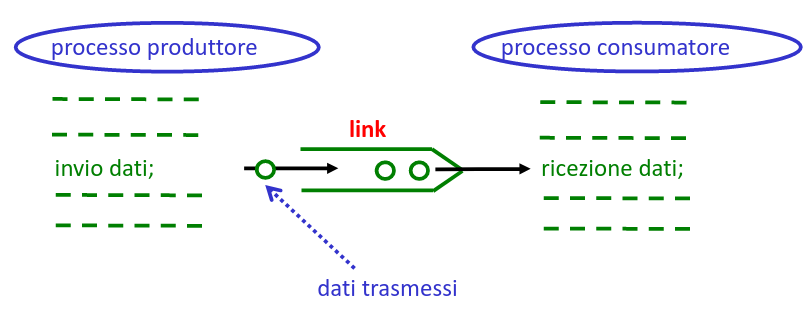
\includegraphics[width=1\textwidth]{/home/riccardoob/appunti/linguaggi/images/39.png}
    \end{multicolfigure}
\end{multicols}

\section{Valutatore}
Il valutatore incorpora la funziona di valutazione, che deve \textbf{visitare} l'albero applicando la corretta \textit{semantica} a seconda del nodo visitato.

\subsection{Implementazione}
É necessario implementare un metodo \texttt{eval()} che calcola il valore di una espressione, conviene introdurre questo metodo nella classe astratta dell'AST, per poi specializzare la sua implementazione per ogni tipo di nodo.

\begin{lstlisting}[language=java]
    public abstract class Exp {
       public abstract int eval();
    }
\end{lstlisting}

Si utilizza quindi una metodologia completamente object oriented, senza creare una funzione piena di if..else per scegliere l'azione da eseguire, questo approccio comporta tuttavia la decentralizzazione della valutazione, con conseguente impatto in caso di necessità di modifiche.

\subsubsection{Stile a oggetti}
\begin{lstlisting}[language=java]
    abstract class Exp {
        abstract public int eval();
    }
    ...
    class PlusExp extends OpExp {
        public PlusExp(Exp l, Exp r) {
            super(l,r);
        }
        public String myOp() {
            return "+";
        }
        public int eval() {
            return left.eval() + right.eval();
        }
    }
    ...
    class NumExp extends Exp {
        int val;
        public NumExp(int v) {
            val = v;
        }
        public int eval() {
            return val;
        }
    }
\end{lstlisting}

\subsubsection{Confronto}
\begin{itemize}
    \item Metodologia \textbf{funzionale}
    \begin{itemize}
        \item \textit{PRO}: facilitata l'introduzione di \textbf{nuove interpretazioni}, basta scrivere una nuova \texttt{eval2()}
        \item \textit{CONTRO}: rende più oneroso introdurre una \textbf{nuova produzione}, impatta tutte le funzioni di interpretazione
    \end{itemize}
    \item Metodologia \textbf{object oriented}
    \begin{itemize}
        \item \textit{PRO}: facilita l'aggiunta di \textbf{nuove produzioni}, basta aggiungere nuova classe, con relative eval
        \item \textit{CONTRO}: rende oneroso introdurre \textbf{nuove intepretazioni}, impatta tutte le classi della tassonomia nell'introduzione del relativo metodo
    \end{itemize}
\end{itemize}

\subsubsection{Cosa scegliere}
Solitamente un linguaggio di programmazione ha una \textit{grammatica fissa} ma richiede \textit{molteplici interpretazioni} delle frasi (per analisi della semantica, type checking, code generation etc.); per questo l'approccio funzionale sembrerebbe il più adatto.

É necessario unire i pro delle due metodologie, a questo compito si presta perfettamente il \textbf{pattern Visitor}, che ci permette di incapsulare la \textit{logica d'interpretazione} in una entità di livello più alto.

\subsection{Visitor come interprete}
Questo pattern realizza la logica di interpretazione in modo coerente all'approccio a oggetti: cattura \textbf{una} logica di interpretazione, centralizzandola in un unico posto.

Nel caso delle espressioni si possono realizzare
\begin{itemize}
    \item una classe base astratta (o interfaccia) \texttt{Visitor}
    \item visitor per \textit{stampare} le espressioni $\rightarrow$ \texttt{ParExpVisitor}
    \item visitor per \textit{calcolare} le espressioni $\rightarrow$ \texttt{EvalVisitor}
    \item visitor per tradurre le espressioni sotto forma di \textit{codice}
    \item ...
\end{itemize}

\begin{multicols}{2}
    \begin{multicolfigure}
        \centering
        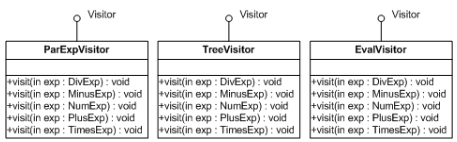
\includegraphics[width=1\textwidth]{/home/riccardoob/appunti/linguaggi/images/41.png}
    \end{multicolfigure}
    \begin{multicolfigure}
        \centering
        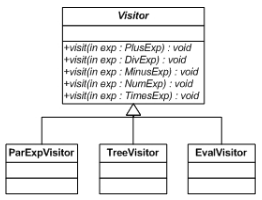
\includegraphics[width=0.7\textwidth]{/home/riccardoob/appunti/linguaggi/images/42.png}
    \end{multicolfigure}
    
\end{multicols}

\textbf{\_\_\_\_\_\_\_\_\_\_\_\_\_\_\_\_\_\_\_\_\_\_\_\_\_\_\_\_\_\_\_\_\_\_\_\_\_\_\_\_\_\_\_\_\_\_\_\_\_\_\_inserisci codice slide 162-173\_\_\_\_\_\_\_\_\_\_\_\_\_\_\_\_\_\_\_\_\_\_\_\_\_\_\_\_\_\_\_\_\_\_\_\_\_\_\_\_\_\_\_\_\_\_\_\_\_\_\_}
























